\section{BinaryGWatch}
\subsection{PCB}
The PCB is based on the Binary Watch. Even the Buttons would still work if soldered on the board. Additionally to the original Schematics there is a Bosch BMA456 connected to the SPI, which is already on the back of the PCB to enable programming via Pogo Pins. Additionally there is also the Chip select pin used and two interrupt pins to enable the wakeup functionality via the BMA sensor. 

The SPI interface was chosen, to keep thepower consumption low, since SPI compared to I2C doesn't need PullUp Resistors.

The BMA Sensor is mounted on the back of the PCB to keep the symetric watch face.

The concept is to use the BMA Sensor also as interface. To enable the Display and also to set the time. So no buttons will be needed this should also enable a housing without holes to keep sweat from crawling into and solve the corroded PCB problems I had with the first BinaryWatch
\subsection{Software}
For interfacing with the BMA i use my own \href{https://github.com/sulkith/Bosch_BMA456}{Bosch\_BMA456} with an additional SPI-adapter.

The Software still has the ability to work with Buttons, but since the BMA is working really well there is no point in using th buttons. and risking that sweat will enter the housing.
\subsection{Housing}
Adapting the housing was very easy, just remove the holes for the buttons.
A little smoothing was done afterwards, because there were some thickened walls around the holes, where the Buttons were mounted.
\subsection{Manual}
\subsubsection{How to read the Watch}
The time is displayed in BCD Code. For further reference please see the Picture below:
\begin{center}
  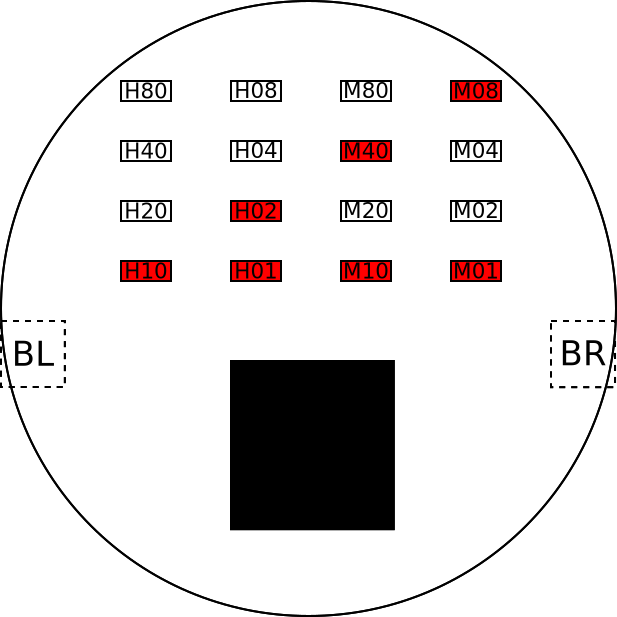
\includegraphics[width=0.5\textwidth]{drawings/BinDia1359.png}
\label{fig:BinWatchFace}
\end{center}
To read the Watch it is necessary to activate the Display this can be either done via double tapping the Housing or raising the arm to take a look on the watch(tilt it by a minimum of 12 degrees with the Watchface facing up and holding it steady for about one second)

The LEDs are read columnwise. So the right two columns are showing the Minutes. If an LED is litone have to add its Value to the Minutes if not then nothing is added. So for the full hour no led in the right two columns will be lit.

In the Example above the following LEDs are lit: M40, M10, M08 and M01.
The sum of all the values is the current minute value $40+10+8+1=59$

The Hours are displayed exactly like the Minutes. For the hours the 24 Hour Format is used. In the Example above the following LEDs are lit: H10, H01, H02. The current Hour Value is also determined by summing everythin up: $10+1+2=13$.

So the current Time in the example is 13:59. If it is 0:00 the watch will display 24:00 to make sure 0:00 is not confused with a broken watch.
\subsubsection{set the time}
To set the time first of all the display has to be activated, afterwards the watchface needs to be turned down and double tapping the Housing.
If the First step was succesful the two LEDs H80 and M80 will light up together. To enter the set hour mode the watchface needs to be turned up again and the watch needs to be double tapped again.

Now the LED M80 will be turned off.

To change the Value the watch needs to be tilted up to increase the value or tilted down to decrease the value, to switch to set minute mode the watch needs to be double tapped again. Changing the minutes works exactly like changing hours. To finish the setup process double tap the cloak again. Now the second counter will also start with zero, so it is possible to set the time precisely.